\documentclass[9pt]{beamer}  % Set document class to Beamer with 9pt font size
\usetheme{metropolis}  % Set theme for the presentation (Warsaw theme)
\usecolortheme{default}  % Set color theme for the presentation (sidebar tab style)
\usepackage[utf8]{inputenc}  % Set input encoding to UTF-8 for proper character handling
\usepackage{graphicx} % Include graphicx package for image handling


\usepackage{epsfig}
%\usepackage[colorlinks=true, urlcolor=blue, linkcolor=red]{hyperref}
\usepackage{tikz, adjustbox}
\usepackage[most]{tcolorbox}
\usepackage{xcolor}
\usepackage{wrapfig}
\usepackage{multicol}

%................................................................
%           Defining colors for sticky notes:
%_______________________________________________________________
% Yellow:
\definecolor{BgYellow}{HTML}{FFF59C}
\definecolor{FrameYellow}{HTML}{F7A600}
% Pink:
\definecolor{BgPink}{HTML}{EF6FA7}
\definecolor{FramePink}{HTML}{E5446E}
% Green:
\definecolor{BgGreen}{HTML}{C7D92D}
\definecolor{FrameGreen}{HTML}{89B23B}
% Blue:
\definecolor{BgBlue}{HTML}{45BEE9}
\definecolor{FrameBlue}{HTML}{31A8C9}
% White:
\definecolor{BgWhite}{HTML}{D8D8D8}
\definecolor{FrameWhite}{HTML}{7F7F7F}
% Brown:
\definecolor{BgBrown}{HTML}{8E7A45}
\definecolor{FrameBrown}{HTML}{6B5B32}
%................................................................
%                   NB command:
%_______________________________________________________________
\usepackage{contour}
\newcommand{\NB}{\contour{black}{\textbf{{\large\sffamily\color{red}NB}}}\textbf{\large\sffamily: }}
%................................................................
%
%               Defining Sticky note boxes:
%_______________________________________________________________
% Yellow Sticky Note (YStkyNote):
\newtcolorbox{YStkyNote}[1][]{%
    enhanced,
    before skip=5mm,after skip=5mm, 
    width=0.7\textwidth, % width of the sticky note
    boxrule=0.2mm,
    colback=BgYellow, colframe=FrameYellow, % Colors
    attach boxed title to top left={xshift=0cm,yshift*=0mm-\tcboxedtitleheight},
    varwidth boxed title*=-3cm,
    % The titlebox:
    boxed title style={frame code={%
        \path[left color=FrameYellow,right color=FrameYellow,
        middle color=FrameYellow]
        ([xshift=-0mm]frame.north west) -- ([xshift=0mm]frame.north east)
        [rounded corners=0mm]-- ([xshift=0mm,yshift=0mm]frame.north east)
        -- (frame.south east) -- (frame.south west)
        -- ([xshift=0mm,yshift=0mm]frame.north west)
        [sharp corners]-- cycle;
        },interior engine=empty,
    },
    sharp corners,rounded corners=southeast,arc is angular,arc=3mm,
    % The "folded paper" in the bottom right corner:
    underlay={%
        \path[fill=BgYellow!80!black] ([yshift=3mm]interior.south east)--++(-0.4,-0.1)--++(0.1,-0.2);
        \path[draw=FrameYellow,shorten <=-0.05mm,shorten >=-0.05mm,color=FrameYellow] ([yshift=3mm]interior.south east)--++(-0.4,-0.1)--++(0.1,-0.2);
        },
    drop fuzzy shadow, % Shadow
    fonttitle=\bfseries, 
    title={#1}
}

% Pink Sticky Note (PStkyNote):
\newtcolorbox{PStkyNote}[1][]{%
    enhanced,
    before skip=2mm,after skip=2mm, 
    width=0.4\textwidth, % width of the sticky note
    boxrule=0.2mm, 
    colback=BgPink, colframe=FramePink, % Colors
    attach boxed title to top left={xshift=0cm,yshift*=0mm-\tcboxedtitleheight},
    varwidth boxed title*=-3cm,
    % The titlebox:
    boxed title style={frame code={%
        \path[left color=FramePink,right color=FramePink,
        middle color=FramePink]
        ([xshift=-0mm]frame.north west) -- ([xshift=0mm]frame.north east)
        [rounded corners=0mm]-- ([xshift=0mm,yshift=0mm]frame.north east)
        -- (frame.south east) -- (frame.south west)
        -- ([xshift=0mm,yshift=0mm]frame.north west)
        [sharp corners]-- cycle;
        },interior engine=empty,
    },
    sharp corners,rounded corners=southeast,arc is angular,arc=3mm,
    % The "folded paper" in the bottom right corner:
    underlay={%
        \path[fill=BgPink!80!black] ([yshift=3mm]interior.south east)--++(-0.4,-0.1)--++(0.1,-0.2);
        \path[draw=FramePink,shorten <=-0.05mm,shorten >=-0.05mm,color=FramePink] ([yshift=3mm]interior.south east)--++(-0.4,-0.1)--++(0.1,-0.2);
        },
    drop fuzzy shadow, % Shadow
    fonttitle=\bfseries, 
    title={#1}
}
% Green Sticky Note (GStkyNote):
\newtcolorbox{GStkyNote}[1][]{%
    enhanced,
    before skip=2mm,after skip=2mm, 
    width=0.4\textwidth, % width of the sticky note
    boxrule=0.2mm,
    colback=BgGreen, colframe=FrameGreen, % Colors
    attach boxed title to top left={xshift=0cm,yshift*=0mm-\tcboxedtitleheight},
    varwidth boxed title*=-3cm,
    % The titlebox:
    boxed title style={frame code={%
        \path[left color=FrameGreen,right color=FrameGreen,
        middle color=FrameGreen]
        ([xshift=-0mm]frame.north west) -- ([xshift=0mm]frame.north east)
        [rounded corners=0mm]-- ([xshift=0mm,yshift=0mm]frame.north east)
        -- (frame.south east) -- (frame.south west)
        -- ([xshift=0mm,yshift=0mm]frame.north west)
        [sharp corners]-- cycle;
        },interior engine=empty,
    },
    sharp corners,rounded corners=southeast,arc is angular,arc=3mm,
    % The "folded paper" in the bottom right corner:
    underlay={%
        \path[fill=BgGreen!80!black] ([yshift=3mm]interior.south east)--++(-0.4,-0.1)--++(0.1,-0.2);
        \path[draw=FrameGreen,shorten <=-0.05mm,shorten >=-0.05mm,color=FrameGreen] ([yshift=3mm]interior.south east)--++(-0.4,-0.1)--++(0.1,-0.2);
        },
    drop fuzzy shadow, % Shadow
    fonttitle=\bfseries, 
    title={#1}
}
% Blue Sticky Note (BStkyNote):
\newtcolorbox{BStkyNote}[1][]{%
    enhanced,
    before skip=2mm,after skip=2mm, 
    width=0.4\textwidth, % width of the sticky note
    boxrule=0.2mm,
    colback=BgBlue, colframe=FrameBlue, % Colors
    attach boxed title to top left={xshift=0cm,yshift*=0mm-\tcboxedtitleheight},
    varwidth boxed title*=-3cm,
    % The titlebox:
    boxed title style={frame code={%
        \path[left color=FrameBlue,right color=FrameBlue,
        middle color=FrameBlue]
        ([xshift=-0mm]frame.north west) -- ([xshift=0mm]frame.north east)
        [rounded corners=0mm]-- ([xshift=0mm,yshift=0mm]frame.north east)
        -- (frame.south east) -- (frame.south west)
        -- ([xshift=0mm,yshift=0mm]frame.north west)
        [sharp corners]-- cycle;
        },interior engine=empty,
    },
    sharp corners,rounded corners=southeast,arc is angular,arc=3mm,
    % The "folded paper" in the bottom right corner:
    underlay={%
        \path[fill=BgBlue!80!black] ([yshift=3mm]interior.south east)--++(-0.4,-0.1)--++(0.1,-0.2);
        \path[draw=FrameBlue,shorten <=-0.05mm,shorten >=-0.05mm,color=FrameBlue] ([yshift=3mm]interior.south east)--++(-0.4,-0.1)--++(0.1,-0.2);
        },
    drop fuzzy shadow, % Shadow
    fonttitle=\bfseries, 
    title={#1}
}
% White Sticky Note (WStkyNote):
\newtcolorbox{WStkyNote}[1][]{%
    enhanced,
    before skip=2mm,after skip=2mm, 
    width=0.4\textwidth, % width of the sticky note
    boxrule=0.2mm,
    colback=BgWhite, colframe=FrameWhite, % Colors
    attach boxed title to top left={xshift=0cm,yshift*=0mm-\tcboxedtitleheight},
    varwidth boxed title*=-3cm,
    % The titlebox:
    boxed title style={frame code={%
        \path[left color=FrameWhite,right color=FrameWhite,
        middle color=FrameWhite]
        ([xshift=-0mm]frame.north west) -- ([xshift=0mm]frame.north east)
        [rounded corners=0mm]-- ([xshift=0mm,yshift=0mm]frame.north east)
        -- (frame.south east) -- (frame.south west)
        -- ([xshift=0mm,yshift=0mm]frame.north west)
        [sharp corners]-- cycle;
        },interior engine=empty,
    },
    sharp corners,rounded corners=southeast,arc is angular,arc=3mm,
    % The "folded paper" in the bottom right corner:
    underlay={%
        \path[fill=BgWhite!80!black] ([yshift=3mm]interior.south east)--++(-0.4,-0.1)--++(0.1,-0.2);
        \path[draw=FrameWhite,shorten <=-0.05mm,shorten >=-0.05mm,color=FrameWhite] ([yshift=3mm]interior.south east)--++(-0.4,-0.1)--++(0.1,-0.2);
        },
    drop fuzzy shadow, % Shadow
    fonttitle=\bfseries, 
    title={#1}
}
% Brown Sticky Note (BrStkyNote):
\newtcolorbox{BrStkyNote}[1][]{%
    enhanced,
    before skip=2mm,after skip=2mm, 
    width=0.4\textwidth, % width of the sticky note
    boxrule=0.2mm,
    colback=BgBrown, colframe=FrameBrown, % Colors
    attach boxed title to top left={xshift=0cm,yshift*=0mm-\tcboxedtitleheight},
    varwidth boxed title*=-3cm,
    % The titlebox:
    boxed title style={frame code={%
        \path[left color=FrameBrown,right color=FrameBrown,
        middle color=FrameBrown]
        ([xshift=-0mm]frame.north west) -- ([xshift=0mm]frame.north east)
        [rounded corners=0mm]-- ([xshift=0mm,yshift=0mm]frame.north east)
        -- (frame.south east) -- (frame.south west)
        -- ([xshift=0mm,yshift=0mm]frame.north west)
        [sharp corners]-- cycle;
        },interior engine=empty,
    },
    sharp corners,rounded corners=southeast,arc is angular,arc=3mm,
    % The "folded paper" in the bottom right corner:
    underlay={%
        \path[fill=BgBrown!80!black] ([yshift=3mm]interior.south east)--++(-0.4,-0.1)--++(0.1,-0.2);
        \path[draw=FrameBrown,shorten <=-0.05mm,shorten >=-0.05mm,color=FrameBrown] ([yshift=3mm]interior.south east)--++(-0.4,-0.1)--++(0.1,-0.2);
        },
    drop fuzzy shadow, % Shadow
    fonttitle=\bfseries, 
    title={#1}
}
%................................................................
%







% Title Page Information
\title{AMP Volatility Managed Portfolios}  % Set the title of the presentation
\author{Moana Valdenaire, Wiktor Kotwicki, Nicolas Gamboa Alvarez}  % List the authors
\date{30th of November 2024}  % Set the date for the presentation

\begin{document}  % Start the document content

% Title Frame
\begin{frame}
    \titlepage  % Generate the title page
\end{frame}


\begin{frame}{Where are we?}

    \begin{itemize}
        \item Clearly defined the asset class we want to explore
        \item Able to provide the list of commodities we are going to work with 
        \item Created a code library to support our research and findings 
        \item Scheduled regular meetings with the team members
    \end{itemize}


\end{frame}


% Article Reference Frame
\begin{frame}
    \frametitle{Article}  % Set frame title
    % Cite the article with a clickable link
    We have focused for this session on the following article:
    \begin{itemize}
        \item Moreira, A., \& Muir, T. (2017). Volatility-managed portfolios. \textit{The Journal of Finance, 72}(2), 651-688.\hspace{0.2cm}\href{https://doi.org/10.1111/jofi.12423}{https://doi.org/10.1111/jofi.12423}
    \end{itemize}
\end{frame}

% Key Findings Section
\section{Key findings}  % Start a new section for key findings
\begin{frame}
    \frametitle{Key Findings}  % Set frame title
    
    \textbf{Description of Moreira and Muir Paper:}  % Bold heading for description
    \begin{itemize}  % Start itemized list
        \item The first paper to popularize the volatility-timed approach for improving risk-adjusted returns.
        \item Investors reduce risk exposure during periods of high realized volatility and increase it when volatility is low.
        \item Contrasts traditional risk-return trade-off assumptions.
    \end{itemize}

    \vspace{0.5cm}  % Add space between the sections

    \textbf{Key Findings from the Paper:}  % Bold heading for key findings
    \begin{itemize}  % Start itemized list for findings
        \item \textbf{Improvement in Sharpe Ratios:} Higher risk-adjusted returns across portfolios.
        \item \textbf{Resilience in Recession Periods:} Reduced drawdown due to lower exposure during volatile times.
        \item \textbf{Utility Improvements:} Better outcomes for mean-variance investors and long-term wealth accumulation.
        \item \textbf{Expansion of Mean-Variance Frontier:} Broader opportunities for portfolio optimization.
    \end{itemize}
\end{frame}

% Methodology and Data Section
\begin{frame}
    \frametitle{Methodology and Data}  % Set frame title
    
    \textbf{Variance and Volatility Measures:}  % Bold heading for variance and volatility measures
    \begin{itemize}  % Start itemized list
        \item Inverse of the previous month’s realized variance as a primary measure.
        \item Alternatives explored:
        \begin{itemize}  % Nested itemized list for alternatives
            \item Previous month’s realized variance or volatility.
            \item Expected variance and strategies without leverage or with 50\% leverage.
        \end{itemize}
    \end{itemize}
    
    \vspace{0.5cm}  % Add space between the sections
    
    % Formula for volatility-managed portfolios
    \textbf{Volatility-Managed Portfolios Factor Equation:}  % Bold heading for the equation
    \begin{equation*}
    f^{\sigma}_{t+1} = \frac{c}{\hat{\sigma}^2_t(f)} f_{t+1},  % Display equation
    \end{equation*}

    \vspace{0.5cm}  % Add space between the sections

    \textbf{Data and Assets:}  % Bold heading for data and assets
    \begin{itemize}  % Start itemized list for data
        \item Monthly data reduces rebalancing frequency.
        \item Standard Fama-French factors (MKT, SMB, HML, ...) from US datasets.
        \item Robustness tested with credit risk factors, corporate bonds, and currencies.
    \end{itemize}
\end{frame}

% Turnover, Costs, and Challenges Section
\begin{frame}
    \frametitle{Transaction Costs and Other Challenges}  % Set frame title
    
    \textbf{Transaction costs:}  % Bold heading for turnover and costs
    \begin{itemize}  % Start itemized list for turnover and costs
        \item High turnover erodes Sharpe ratio due to transaction costs, especially for illiquid factors (Barroso \& Detzel, 2021).
        \item Frequent rebalancing and high costs challenge practical implementation.
    \end{itemize}

    \vspace{0.5cm}  % Add space between the sections

    \textbf{Broader Implications:}  % Bold heading for broader implications
    \begin{itemize}  % Start itemized list for broader implications
        \item Best performance during high-sentiment periods, but market conditions limit robustness.
    \end{itemize}

    \vspace{0.5cm}  % Add space between the sections

    \textbf{Practical Challenges:}  % Bold heading for practical challenges
    \begin{itemize}  % Start itemized list for practical challenges
        \item Look-ahead bias and instability lead to underperformance (Cederburg, O’Doherty, \& Jiang, 2020).
        \item High transaction costs and sentiment dependence limit long-term success (Barroso \& Detzel, 2021).
    \end{itemize}
\end{frame}

% Discussion and Future Research Section
\begin{frame}
    \frametitle{Discussion and Future Research}  % Set frame title
    
    % Start tcolorbox for discussion and future research
\begin{tcolorbox}[colframe=blue!70, colback=blue!10, coltitle=black, sharp corners=southwest, boxrule=0.9mm, width=1.0\textwidth, enlarge left by=0.22cm, enlarge right by=0.5cm]
    \textbf {Big Picture Question/Idea:}  % Bold heading inside the box
    \begin{itemize}  % Start itemized list inside the box
        \item How can we better account for transaction and turnover costs?
        \item Which commodities offer the best testing ground for these strategies?
        \item Can we define recession indicators tailored to chosen commodities?
        \item What data frequency provides the optimal balance between signal reliability and costs?
    \end{itemize}
\end{tcolorbox}
\end{frame}

% Slide with Image
\begin{frame}
    \frametitle{Visualization I: Gold Prices and Volumes (Daily)}  % Set frame title
    \begin{center}
        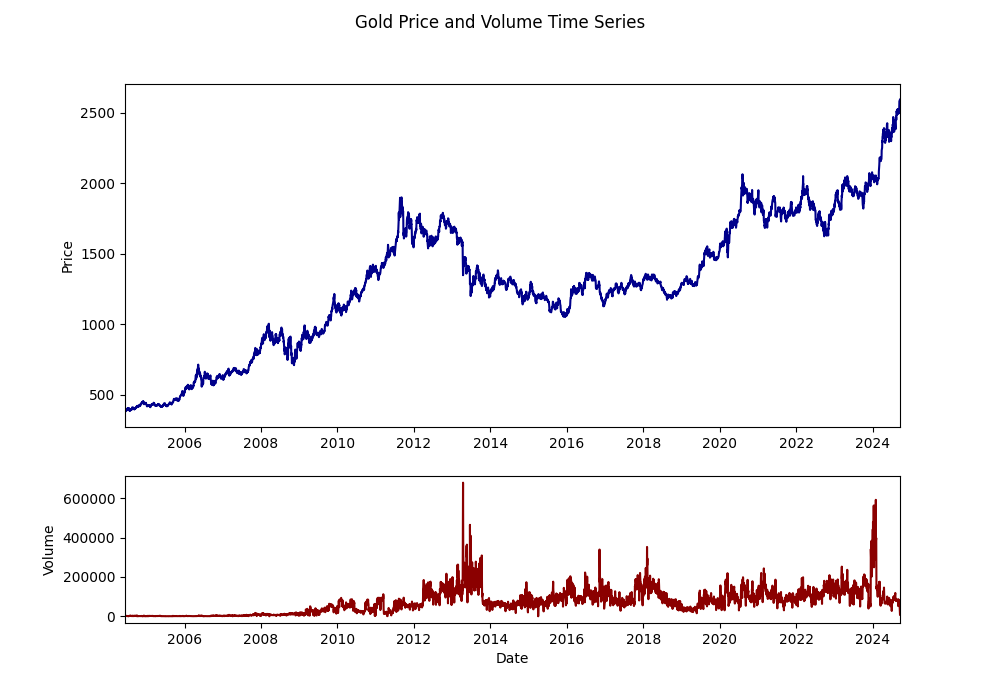
\includegraphics[width=\textwidth, height=0.8\textheight, keepaspectratio]{gold_price_volume.png}  % Include the image with specified width and height
    \end{center}
\end{frame}

% Slide with Image
\begin{frame}
    \frametitle{Visualization II: Gold Returns Volatility (Daily)}  % Set frame title
    \begin{center}
        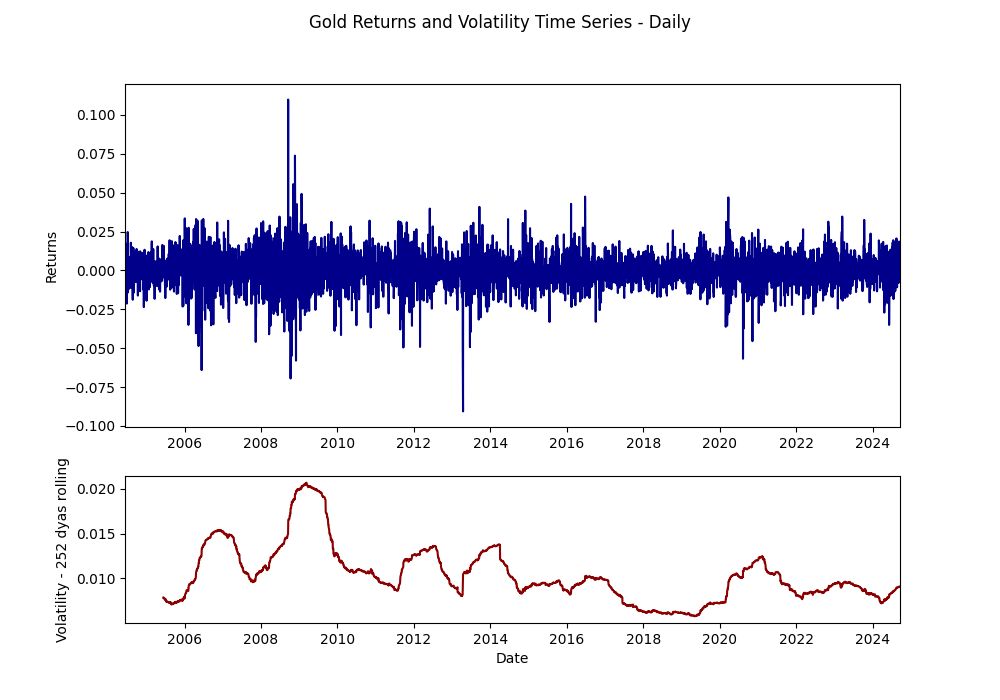
\includegraphics[width=\textwidth, height=0.8\textheight, keepaspectratio]{gold_returns_volatility_daily.png}  % Include the image with specified width and height
    \end{center}
\end{frame}



\begin{frame}{What is next?}
    \begin{YStkyNote}[To do next:]
    \begin{itemize}
        \item Going through more research
        \item Schedule a session in the Bloomberg room
        \item Retrieve and explore historical data from commodities
        \item Building the necessary code to implement portfolio construction dynamics
        \item Continue meeting regularly with the team
    \end{itemize}
    \end{YStkyNote}
\end{frame}

% Slide with Image
\begin{frame}
    \frametitle{What we are building - A code framework}  % Set frame title
    \begin{center}
        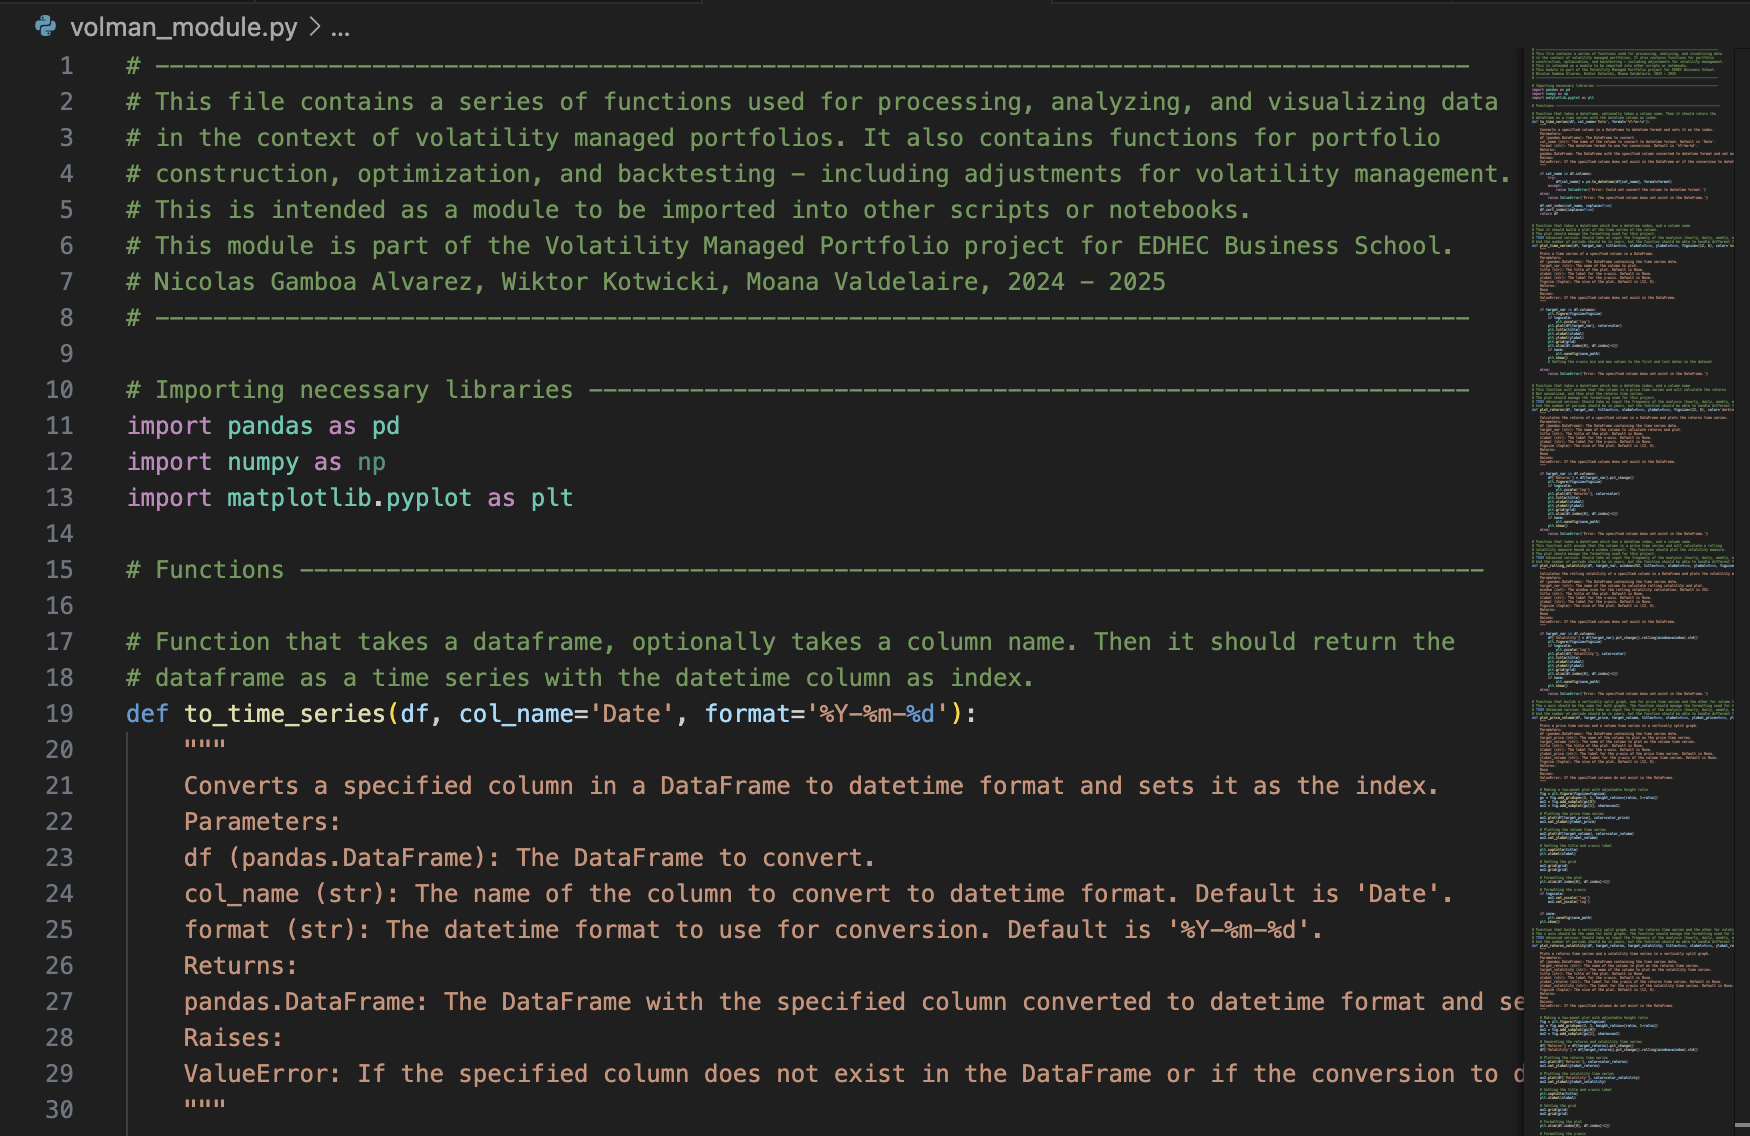
\includegraphics[width=\textwidth, height=0.8\textheight, keepaspectratio]{Screenshot 2024-11-29 at 19.50.18.png}  % Include the image with specified width and height
    \end{center}
\end{frame}

\end{document}  % End the document content